\chapter{Experiments} \label{chap:exp}

In order to evaluate our proposed algorithms, the heuristic balancing method (\emph{GM}), the distance based node clustering scheme (\emph{DIST}), as well as the combination of those (\emph{HDM}), we compare them with the geometric monitoring method~\cite{Sharfman2006GM}, hereby referred to as \emph{GM}, and the hierarchical clustering method of~\cite{Keren2014GMHetStreams}, hereby referred to as \emph{DISTR}. Datasets originate from both synthetic and real-world settings in order to explore the performance, scalability and applicability of our methods in terms of reduction in communication.

Firstly, Section~\ref{sec:datasets} contains a detailed description of the datasets and the monitoring functions used for evaluation purposes. Following that, Section~\ref{sec:exp} presents the experimental results along with the necessary commentation.

\section{Data, Setup and Monitoring Functions} \label{sec:datasets}

\subsection{Synthetic Datasets}

Synthetic datasets have been incorporated into the evaluation process of the proposed algorithms in order to provide a controllable environment under which the behavior of our methods can be analyzed. Data streams are created by firstly sampling data stream velocity distribution means by a user specified normal distribution and fixing the standard deviation of each stream. Afterwards, an initial velocity is sampled from each stream's assigned distribution and a $\lambda$ value is chosen, which controls the rate of change of the streams' velocity. Stream update $v_i(t_k)$ of node $n_i$ at time $t_k$ is generated by sampling a new velocity $u_{k+1}$ from the velocity distribution assigned to node $n_i$ and updating the streams' value by: $v_i(t_{k+1})=v_i(k) + (1-\lambda)u_{k} + \lambda u_{k+1}$. Noisy versions of the generated streams are the product of additive Gaussian noise.

Linear streams (\emph{LIN}) are generated by setting the parent distribution to $\mathcal{N}(10,20)$, the standard deviation of each stream's velocity distribution to $\sigma=10$ and the lambda value to $\lambda=0$. An example of the resulting one dimensional streams corresponding to 20 nodes, along with the resulting global statistics stream, is illustrated in Figure~\ref{fig:linearStreams}.

Interweaving streams(\emph{INT}) are produced from the same parent distribution $\mathcal{N}(10,20)$ by selecting $\sigma=50$ for the standard deviation of each stream's velocity distribution and $\lambda=0.1$ as the velocity update parameter. An instance of one dimensional interweaving streams corresponding to 20 nodes, along with the resulting global statistics stream, is shown in Figure~\ref{fig:intStreams}.

Noisy streams (\emph{NOISE}) are the result of the previously used parent distribution with $\sigma=100$ as the standard deviation of each stream's velocity, $\lambda=0.15$ the velocity update parameter, and  $\mathcal{N}(0,30)$ the distribution of the additive Gaussian noise. Such one dimensional streams corresponding to 20 monitoring nodes, along with the resulting global statistics stream, is depicted in Figure~\ref{fig:noiseStreams}.

%%%%%%%%%%%%%%%%%%%%%%%%%%%%%%%%%LIN synthetic datasets figure %%%%%%%%%%%%%%%%%%%%%%%%%%%%
\begin{figure*}[t!]
\centering
\begin{subfigure}[t]{0.49\textwidth}
\centering
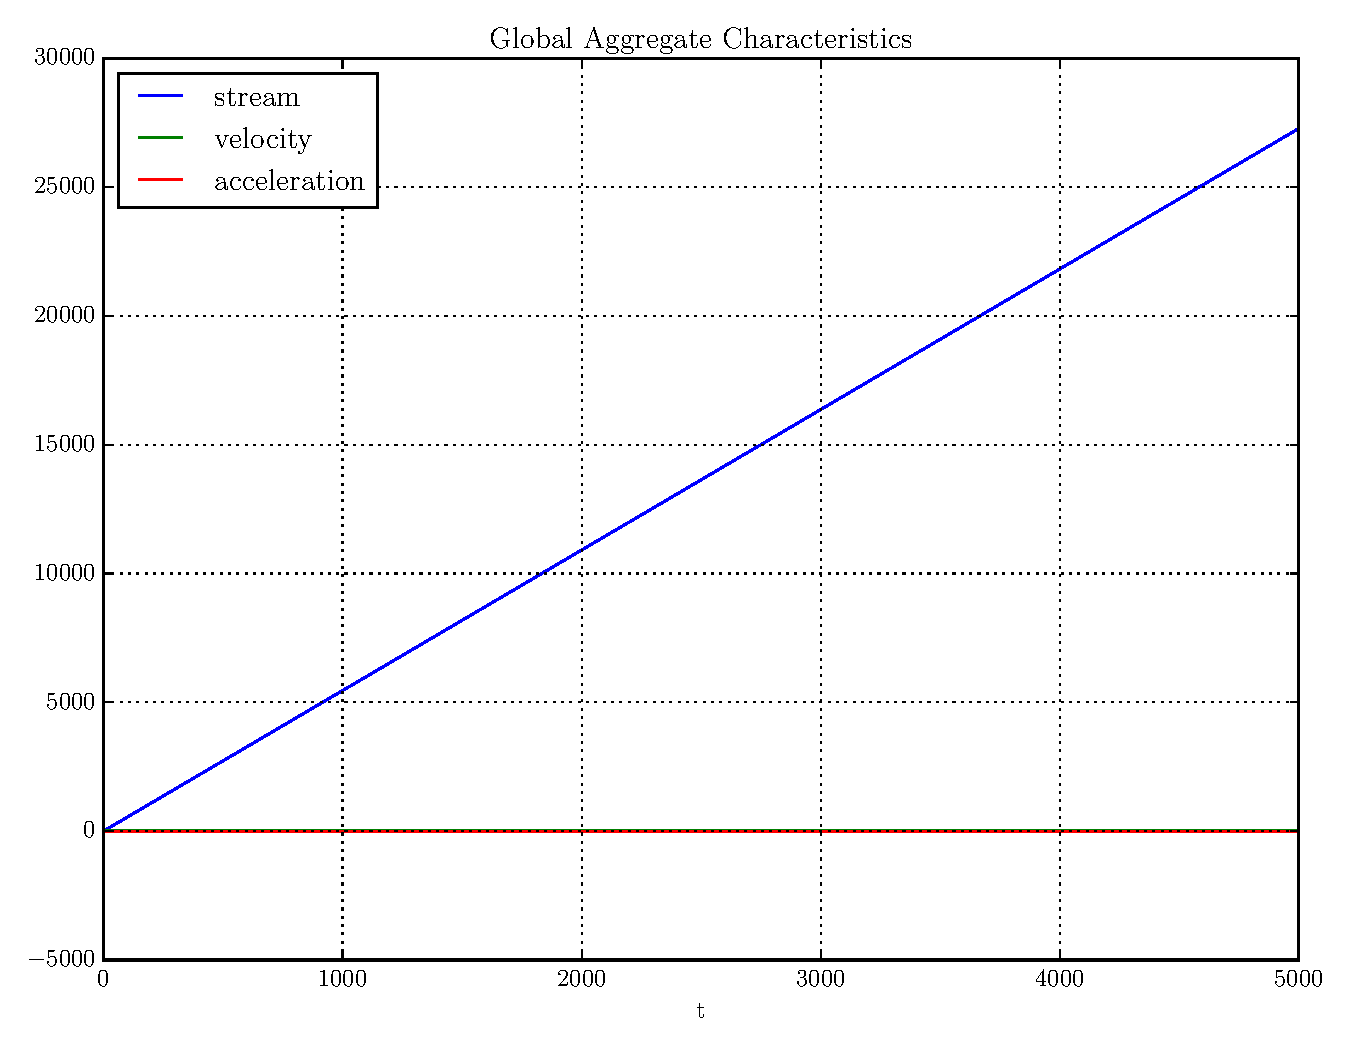
\includegraphics[scale=0.38, trim=2cm 0 0 0]{img/linear1D20N_global.pdf}
\caption{LIN global statistics stream of 20 streams}
\end{subfigure}
\begin{subfigure}[t]{0.49\textwidth}
\centering
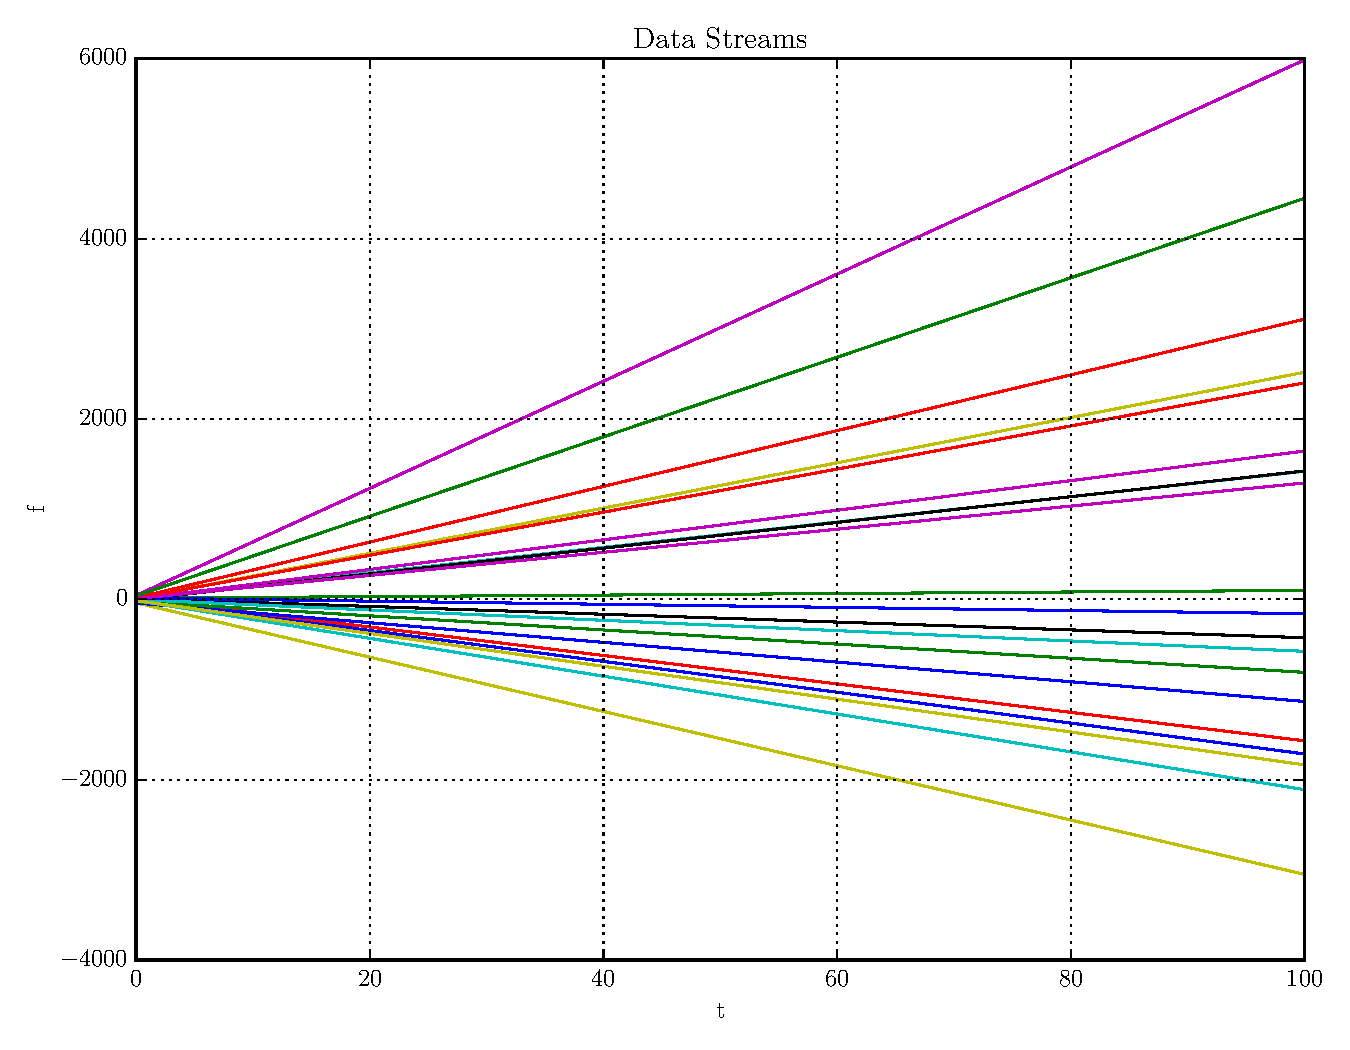
\includegraphics[scale=0.38]{img/linear1D20N_streams.pdf}
\caption{LIN local statistics streams of 20 nodes} 
\end{subfigure}
\vspace{0.5cm}
\caption{Linear data stream examples (LIN)}\label{fig:linearStreams}
\end{figure*}
%%%%%%%%%%%%%%%%%%%%%%%%%%%%%%%%%%%%%%%%%%%%%%%%%%%%%%%%%%%%%%%%%%%%%%%%%%%%%%%%%%%%%%%%%%%

%%%%%%%%%%%%%%%%%%%%%%%%%%%%%%%%%INT synthetic datasets figure %%%%%%%%%%%%%%%%%%%%%%%%%%%%
\begin{figure*}[t!]
\centering
\begin{subfigure}[t]{0.49\textwidth}
\centering
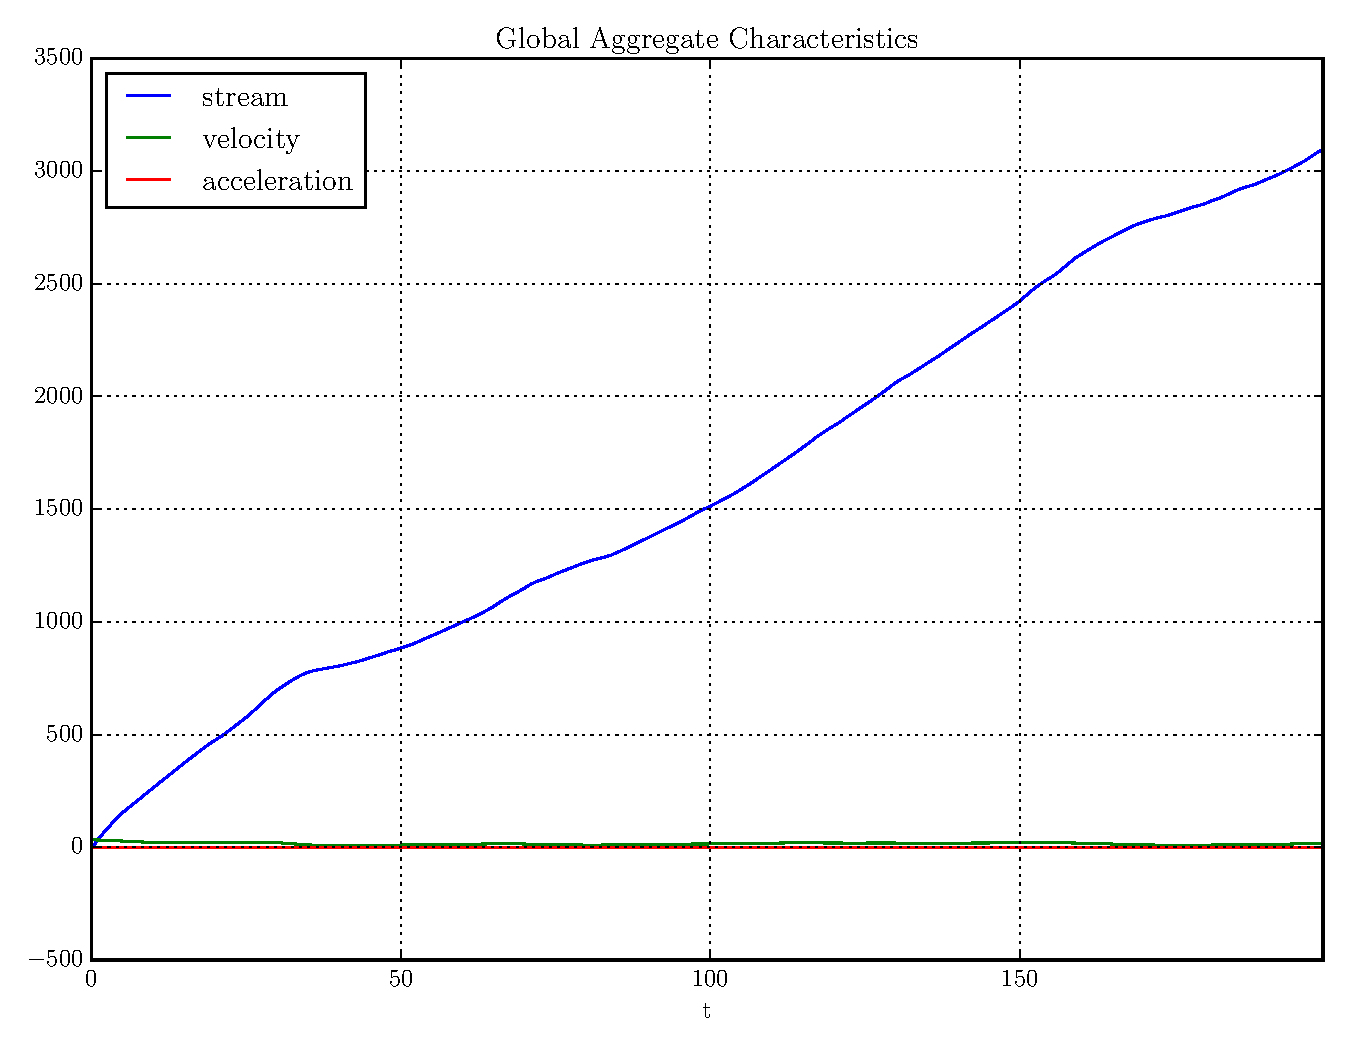
\includegraphics[scale=0.38, trim=2cm 0 0 0]{img/interweaving1D20N_global.pdf}
\caption{INT global statistics stream of 20 streams}
\end{subfigure}
\begin{subfigure}[t]{0.49\textwidth}
\centering
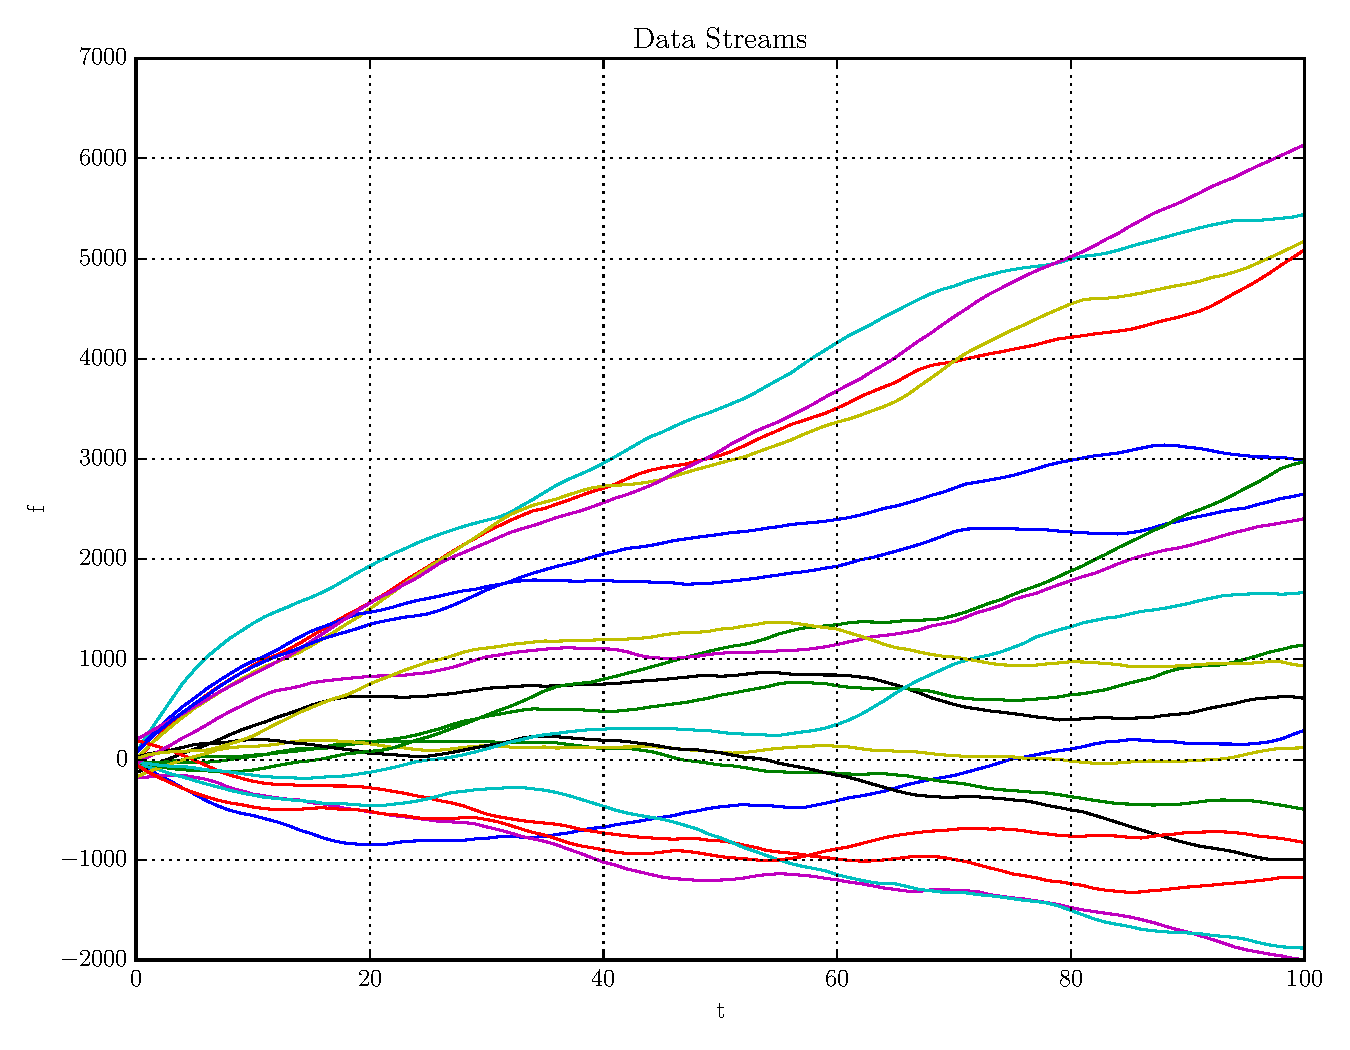
\includegraphics[scale=0.38]{img/interweaving1D20N_streams.pdf}
\caption{INT local statistics streams of 20 nodes} 
\end{subfigure}
\vspace{0.5cm}
\caption{Interweaving data stream examples (INT)}\label{fig:intStreams}
\end{figure*}
%%%%%%%%%%%%%%%%%%%%%%%%%%%%%%%%%%%%%%%%%%%%%%%%%%%%%%%%%%%%%%%%%%%%%%%%%%%%%%%%%%%%%%%%%%%

%%%%%%%%%%%%%%%%%%%%%%%%%%%%%%%%NOISE synthetic datasets figure %%%%%%%%%%%%%%%%%%%%%%%%%%%%
\begin{figure*}[t!]
\centering
\begin{subfigure}[t]{0.49\textwidth}
\centering
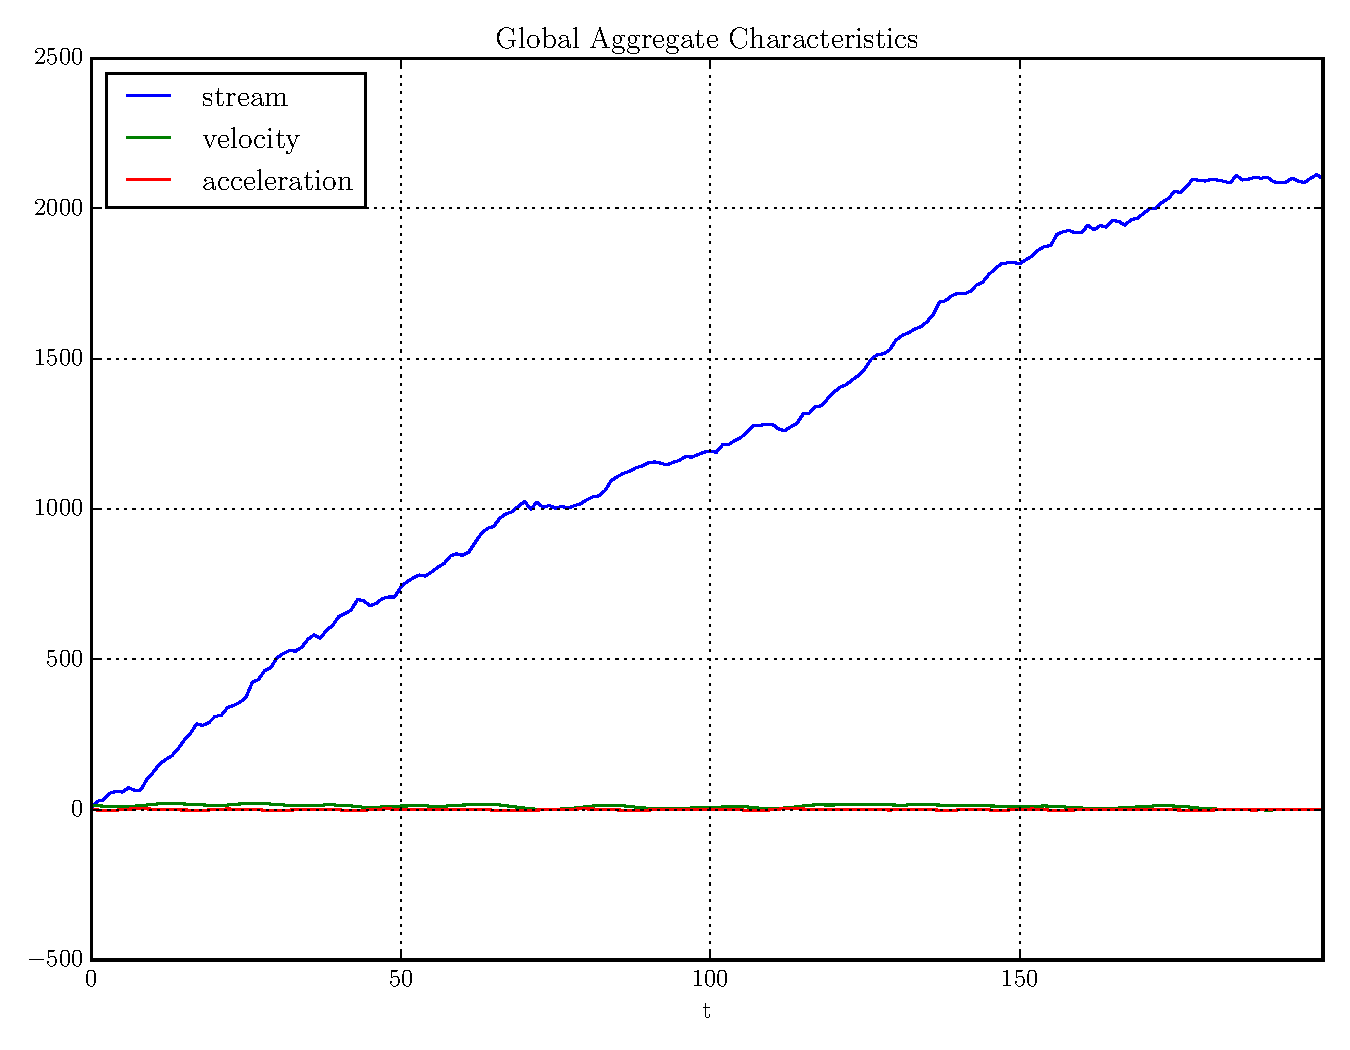
\includegraphics[scale=0.38, trim=2cm 0 0 0]{img/noisyinterweaving1D20N_global.pdf}
\caption{NOISE global statistics stream of 20 streams}
\end{subfigure}
\begin{subfigure}[t]{0.49\textwidth}
\centering
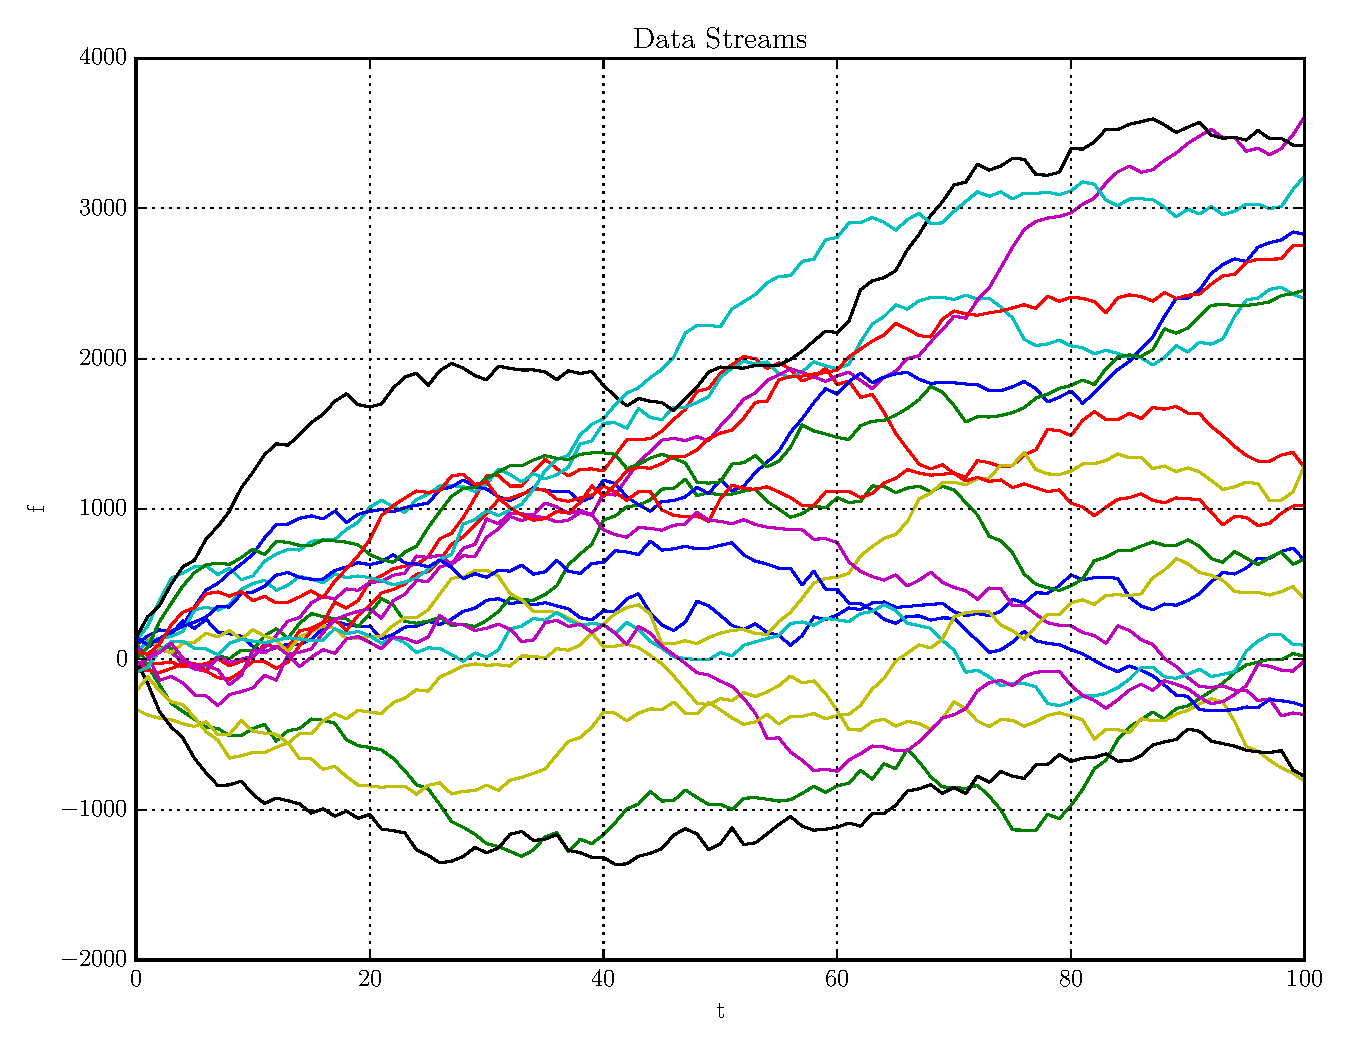
\includegraphics[scale=0.38]{img/noisyinterweaving1D20N_streams.pdf}
\caption{NOISE local statistics streams of 20 nodes} 
\end{subfigure}
\vspace{0.5cm}
\caption{Interweaving data stream examples (NOISE)}\label{fig:noiseStreams}
\end{figure*}
%%%%%%%%%%%%%%%%%%%%%%%%%%%%%%%%%%%%%%%%%%%%%%%%%%%%%%%%%%%%%%%%%%%%%%%%%%%%%%%%%%%%%%%%%%%


%TODO: include actual dataset?
\subsection{Air Quality Database}

The real world dataset consists of measurements of air pollutants, as measured during the year 2014, which can be found in the ``European Environmental Agency - AQ e-Reporting'' database~\cite{AirBase}. Data streams correspond to hourly measurements of air pollutants $NO_2$ and $NO$, in micro-grams per cubic meter, averaged over a window of five days for the whole year. Monitoring nodes are picked at random from available air quality measurement stations across Austria. Notable characteristics of this dataset are the difference in behavior and shape between data streams taken from different stations, and between different air pollutant measurements. These lead to irregularities and great variance between measurements at different time points and locations. Figures~\ref{fig:NO2_sq} and~\ref{fig:NO2_NO} illustrate the global and local statistics streams of 8 nodes that monitor the variance of $NO_2$ pollutant, as well as the ratio of $NO$ to $NO_2$.

%%%%%%%%%%%%%%%%%%%%%%%%%%%%%%%%NO2_sq actual datasets figure %%%%%%%%%%%%%%%%%%%%%%%%%%%%
\begin{figure*}[t!]
\centering
\begin{subfigure}[t]{0.49\textwidth}
\centering
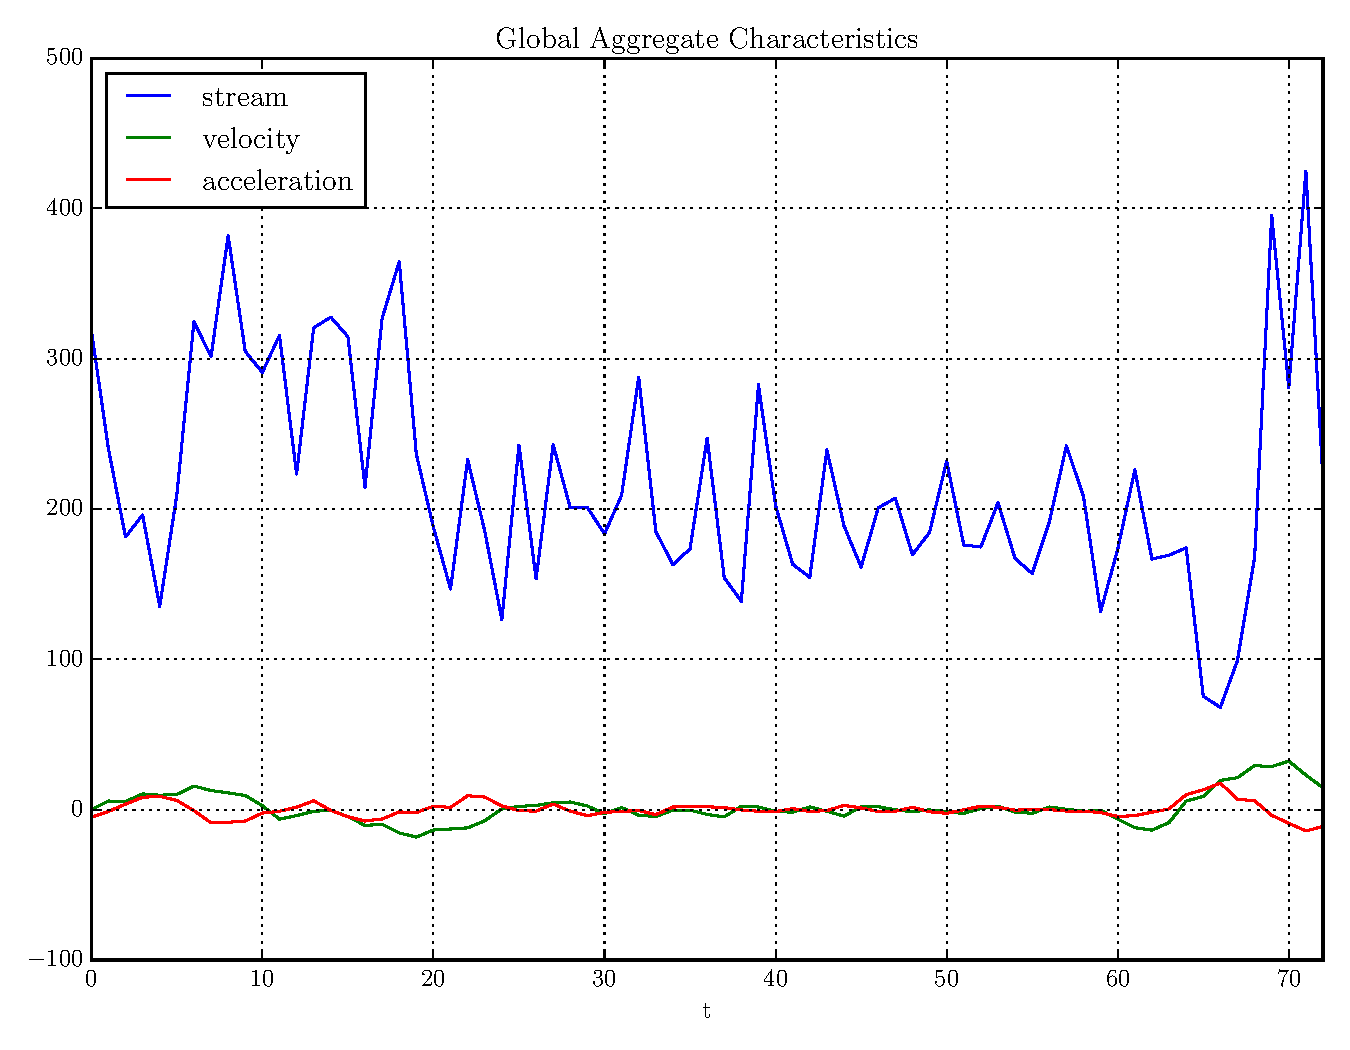
\includegraphics[scale=0.38, trim=2cm 0 0 0]{img/AT_NO2_sq_2014_8N_global.pdf}
\caption{Global statistics stream of 8 nodes monitoring the variance of $NO_2$ air pollutant.}
\end{subfigure}
\begin{subfigure}[t]{0.49\textwidth}
\centering
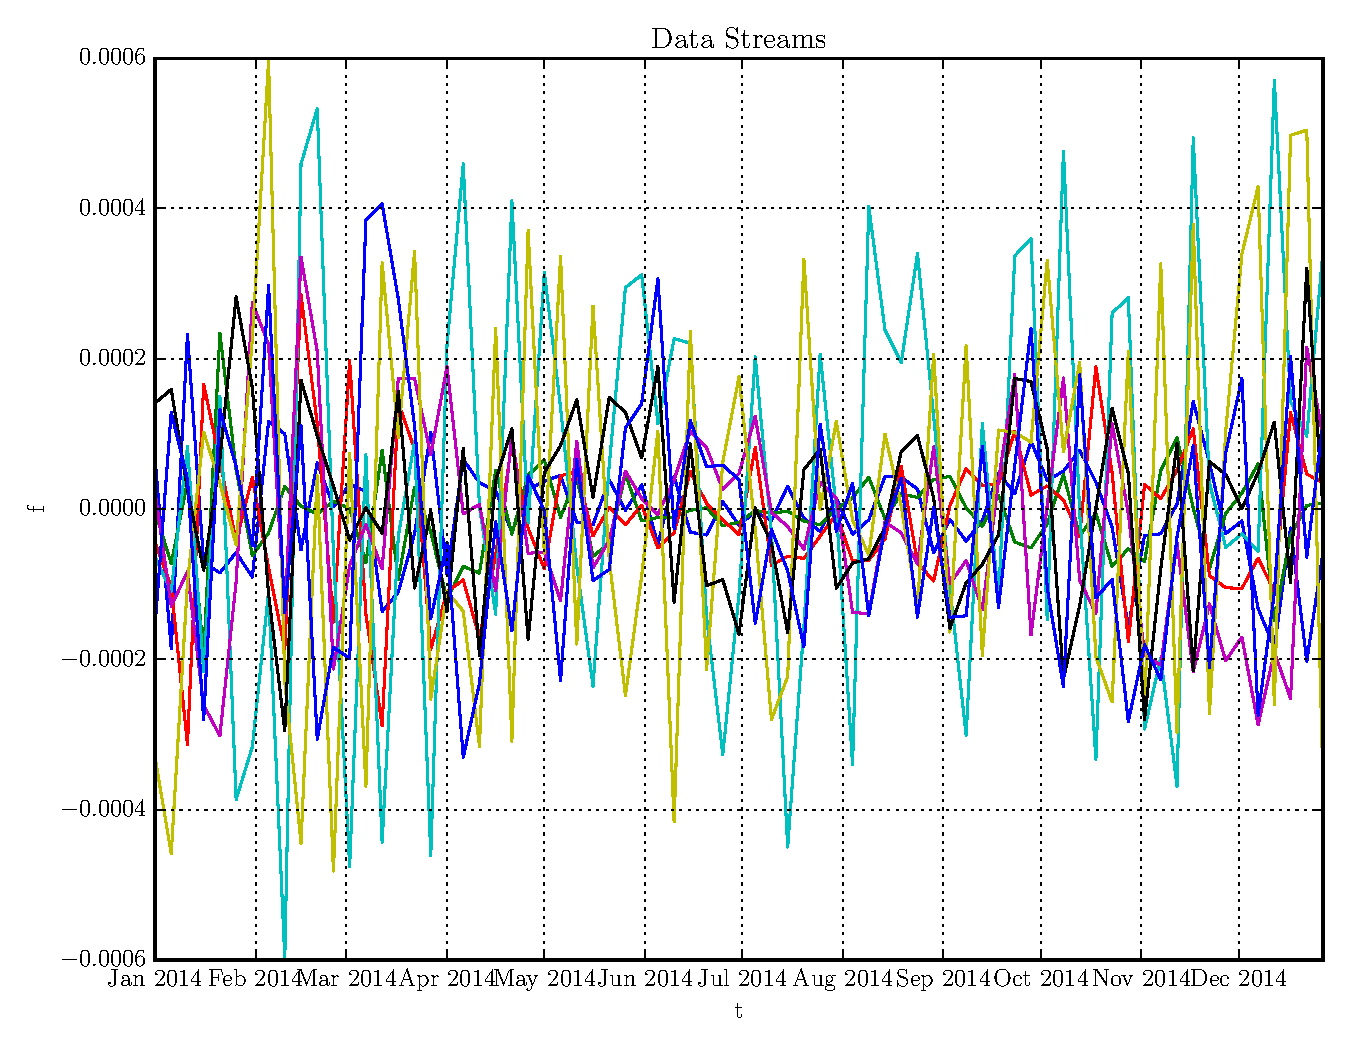
\includegraphics[scale=0.38]{img/AT_NO2_sq_2014_8N_streams.pdf}
\caption{Local statistics streams of 8 nodes monitoring the variance of $NO_2$ air pollutant.} 
\end{subfigure}
\vspace{0.5cm}
\caption{Streams of 8 nodes monitoring the variance of $NO_2$ air pollutant.}\label{fig:NO2_sq}
\end{figure*}
%%%%%%%%%%%%%%%%%%%%%%%%%%%%%%%%%%%%%%%%%%%%%%%%%%%%%%%%%%%%%%%%%%%%%%%%%%%%%%%%%%%%%%%%%%%
%%%%%%%%%%%%%%%%%%%%%%%%%%%%%%%%NO2_NO actual datasets figure %%%%%%%%%%%%%%%%%%%%%%%%%%%%%
\begin{figure*}[t!]
\centering
\begin{subfigure}[t]{0.49\textwidth}
\centering
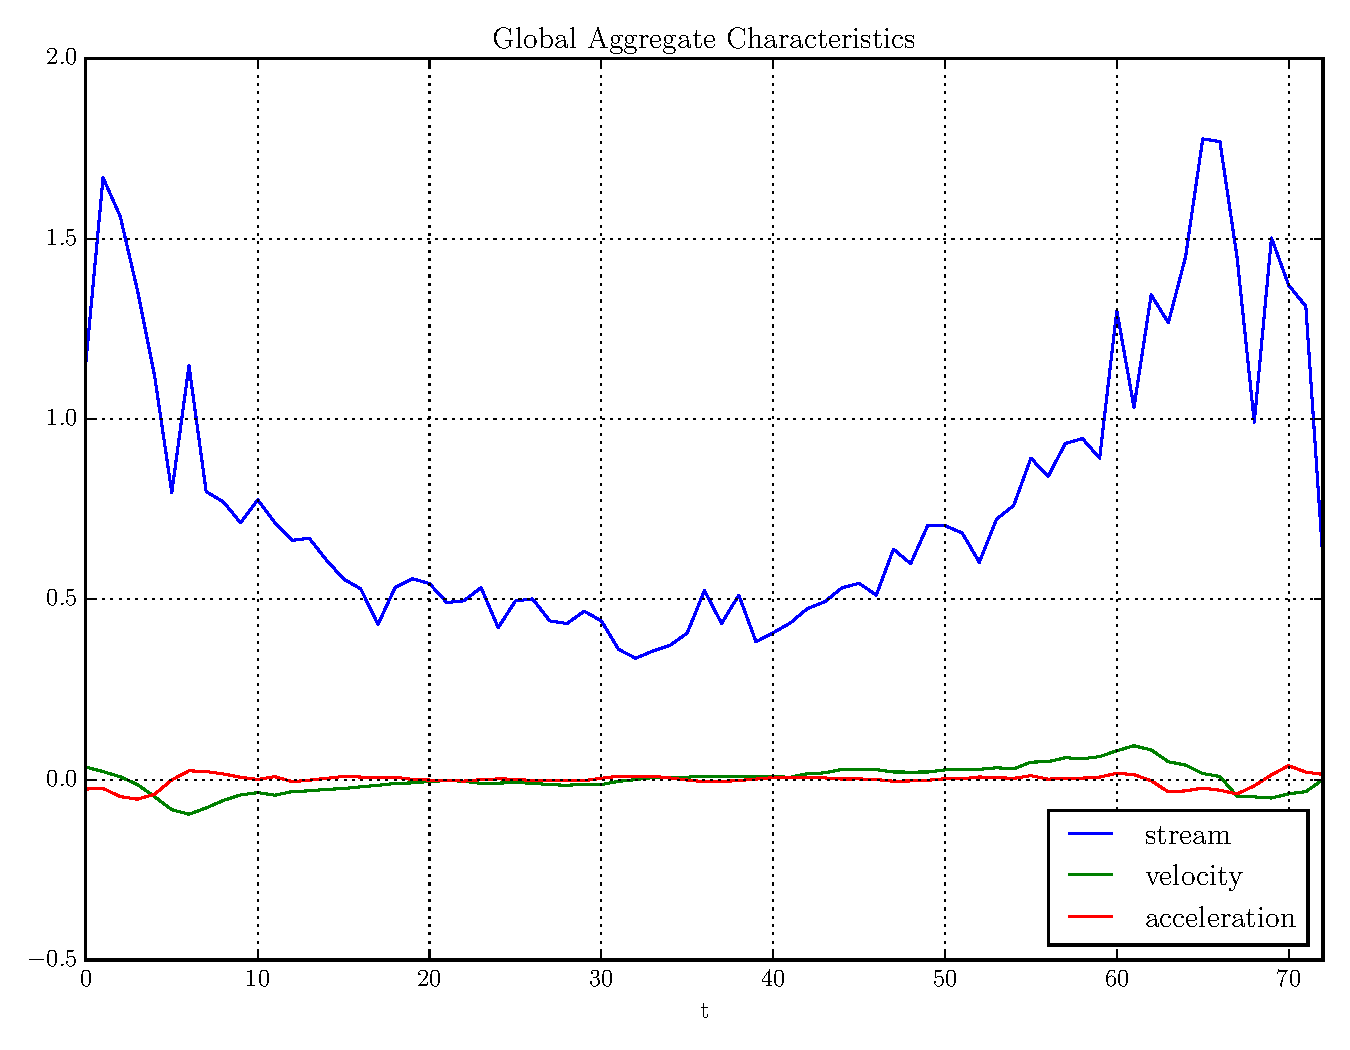
\includegraphics[scale=0.38, trim=2cm 0 0 0]{img/AT_NO2_NO_2014_8N_global.pdf}
\caption{Global statistics stream of 8 nodes monitoring the ratio $NO/NO_2$.}
\end{subfigure}
\begin{subfigure}[t]{0.49\textwidth}
\centering
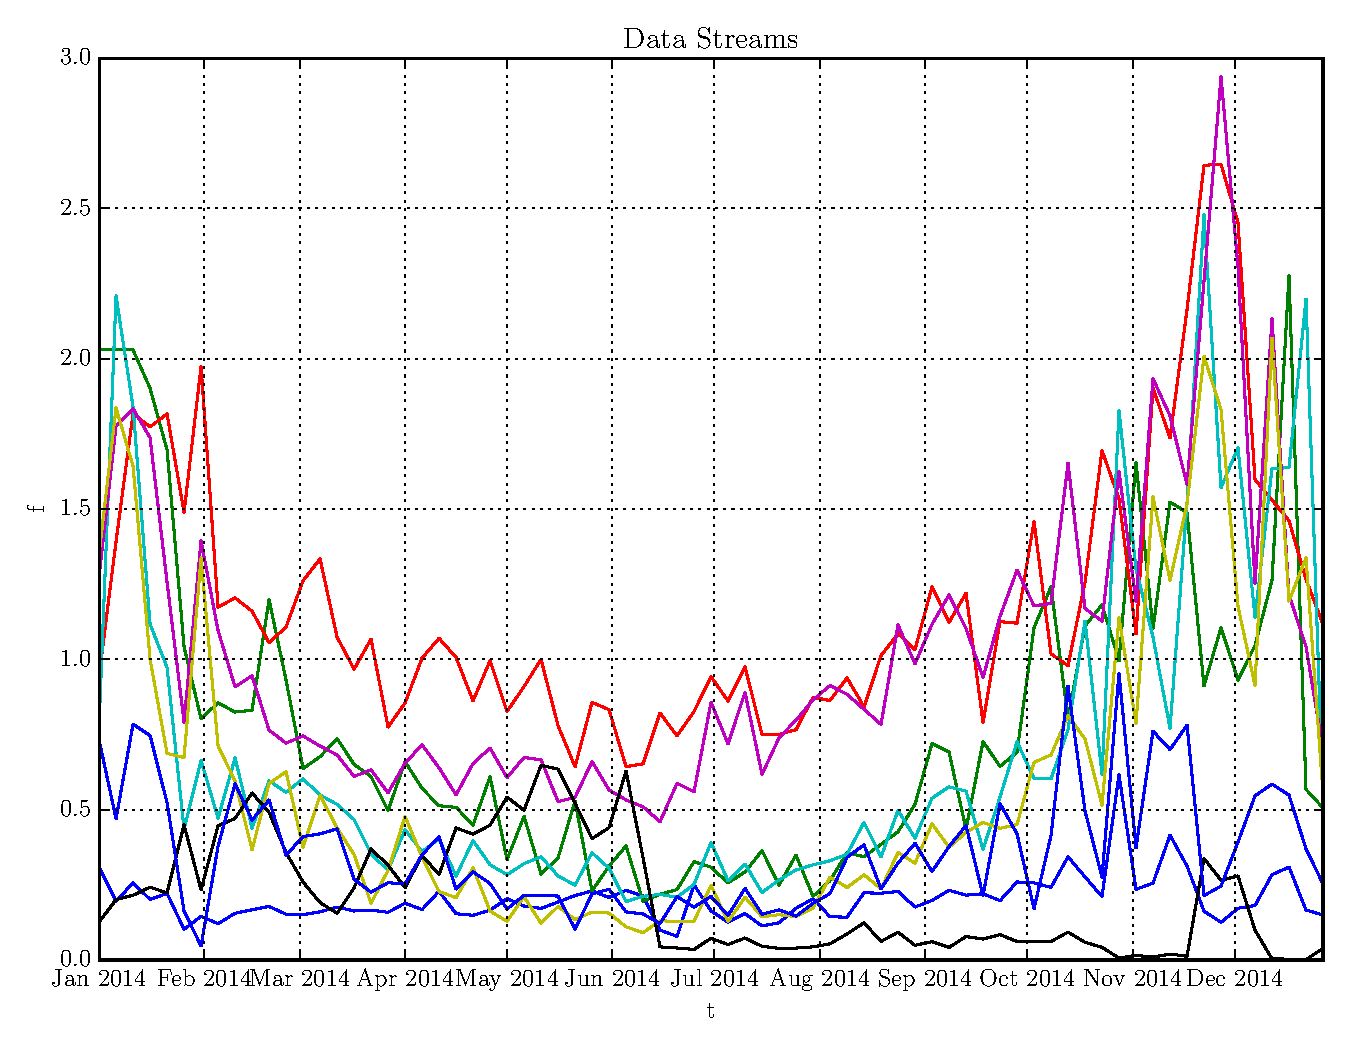
\includegraphics[scale=0.38]{img/AT_NO2_NO_2014_8N_streams.pdf}
\caption{Local statistics streams of 8 nodes monitoring the ratio $NO/NO_2$.} 
\end{subfigure}
\vspace{0.5cm}
\caption{Streams of 8 nodes monitoring the ratio $NO/NO_2$.}\label{fig:NO2_NO}
\end{figure*}
%%%%%%%%%%%%%%%%%%%%%%%%%%%%%%%%%%%%%%%%%%%%%%%%%%%%%%%%%%%%%%%%%%%%%%%%%%%%%%%%%%%%%%%%%%%

\subsection{Monitoring Functions}

The monitoring functions used during the experiments were carefully chosen in order to illustrate, as accurately as possible, the properties and behavior of each examined method. Specifically:
\begin{itemize}
\item Experiments using the one dimensional synthetic datasets (LIN, INT, NOISE) monitor the function $f(x)=x$. This simple functions allows us to clearly examine the behavior of the implemented methods over artificial streams with specific characteristics regarding linearity and noise, without affecting the results.
\item Experiments that incorporate multi-dimensional synthetic datasets (LIN, INT, NOISE) monitor a multi-variable quadratic function $f(x,y,z,k,\dots)=(x-y+z-k+\dots)^2+x+y+z+k+\dots$, with variables $x,y,z,k,\dots$ corresponding to different stream dimensions i.e., a quadratic function with $d$ variables is monitored over $d$-dimensional streams. Quadratic functions are of grave importance to numerous real-world applications (e.g., a Gaussian distribution is expressed via an exponent of a quadratic function).
\item Experiments performed on real-world data streams of air pollutants monitor the variance of $NO_2$ and the ratio of $NO$ to $NO_2$. Both functions operate on two dimensional data. Let $m_{NO_2,t_i}$ and $m_{NO,t_i}$ be measurements of air pollutants $NO_2$ and $NO$ at $t_i$, respectively. The former function operates on data updates $v_{t_i}=\left(\begin{smallmatrix}m_{NO_2,t_i}\\(m_{NO_2,t_i})^2\end{smallmatrix}\right)$ and the latter on data updates $v_{t_i}=\left(\begin{smallmatrix}m_{NO,t_i}\\m_{NO_2,t_i}\end{smallmatrix}\right)$.
\end{itemize}

\section{Experimental Results} \label{sec:exp}

The following experiments are performed in order to gain an insight on the behavior of the methods proposed in this thesis and how these compare to methods presented in prior work, focusing on the communication overhead induced by each method. 

In Subsection~\ref{subsec:matchingComp} our distance based node matching algorithm (Section~\ref{sec:impl-distNodeMatch}) is compared with two methods of violation resolution found in related work. Subsection~\ref{subsec:balComp} compares the balancing algorithm of the seminar work on geometric monitoring with our proposed, heuristic, method. Subsequently, our HDM method is compared with the GM method while exploring the impact different tuning parameters induce on the performance of our algorithm. Finally, our algorithm HDM is put to test using datasets from a real-world domain, with GM operating as the baseline method.

\subsection{Node Matching Algorithms} \label{subsec:matchingComp}

The seminar geometric monitoring method~\cite{Sharfman2006GM} dictates that random nodes are requested in order to perform a violation resolution via the balancing method (RAND). Subsequent work~\cite{Keren2014GMHetStreams} examines the partitioning of nodes into disjoint pairs, so that the probability of a violation resolution in case of a local violation is maximized by maximizing the percentage of data vectors that result to a successful balancing operation (DISTR), either by iterating over all data vectors pairs between all nodes and evaluating the constraint, or by employing the pdfs of the data streams. Our proposed method depends only on simple Euclidean distance computations between data stream vectors, not being bound on the monitoring function and its possible irregularities. All three methods are being compared using the original geometric monitoring balancing method GM.

%%%%%%%%%%%%%%%%%%%%%%%%%%%%%%%%msgs matching lin figure %%%%%%%%%%%%%%%%%%%%%%%%%%%%
\begin{figure*}[t!]
\centering
\begin{subfigure}[t]{0.31\textwidth}
\centering
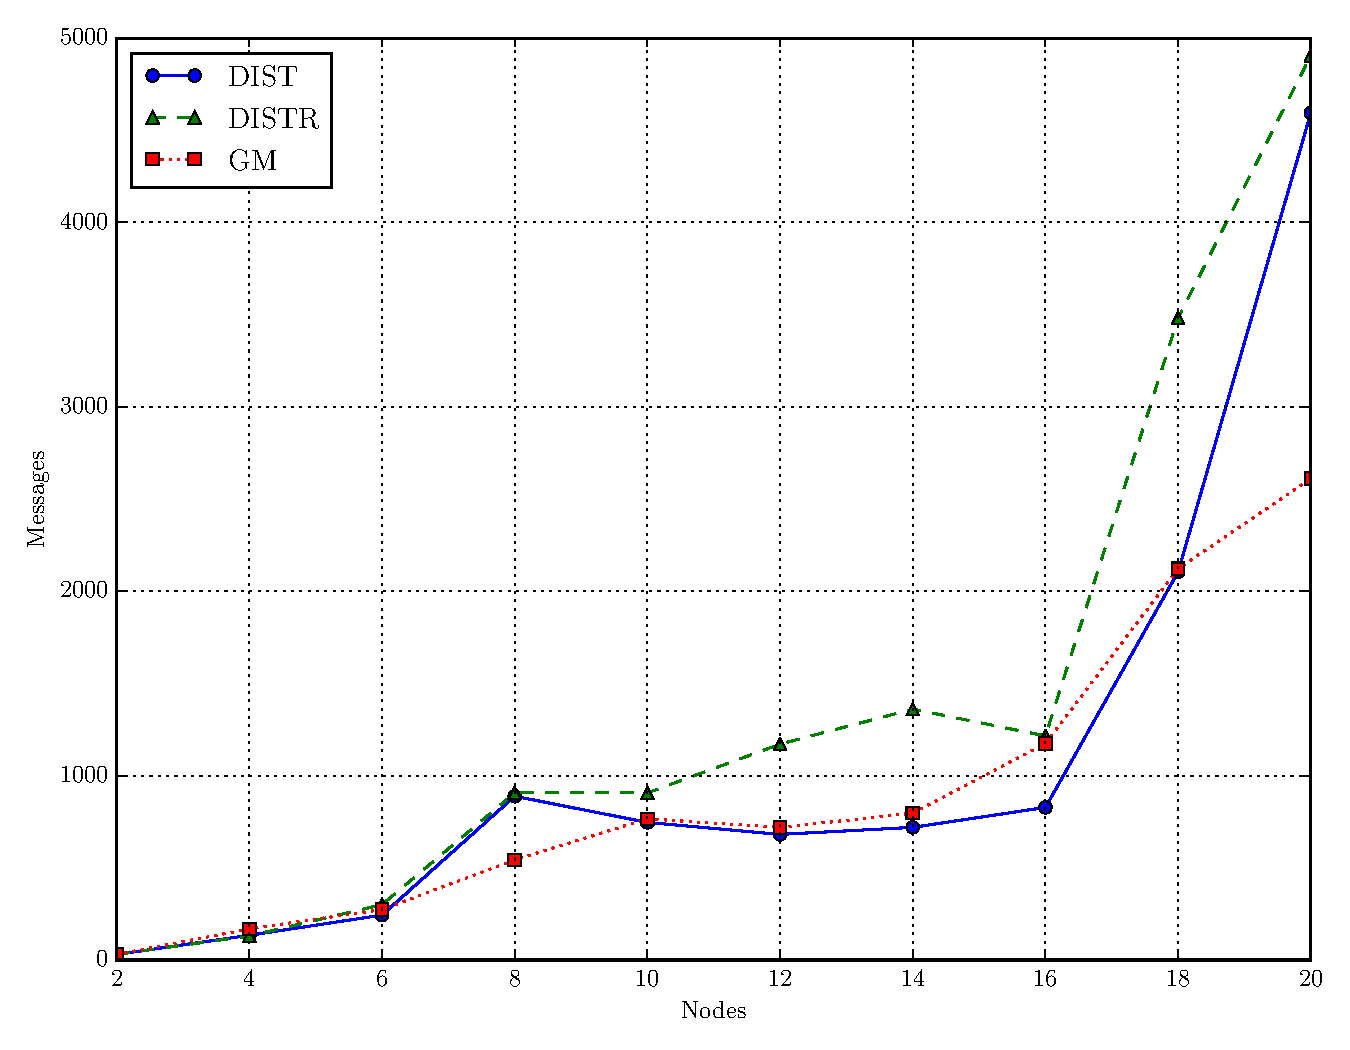
\includegraphics[scale=0.28, trim=10.5cm 0 0 0]{img/matching_msg_linear.pdf}
\caption{Global statistics stream of 8 nodes monitoring the variance of $NO_2$ air pollutant.}
\end{subfigure}
\begin{subfigure}[t]{0.31\textwidth}
\centering
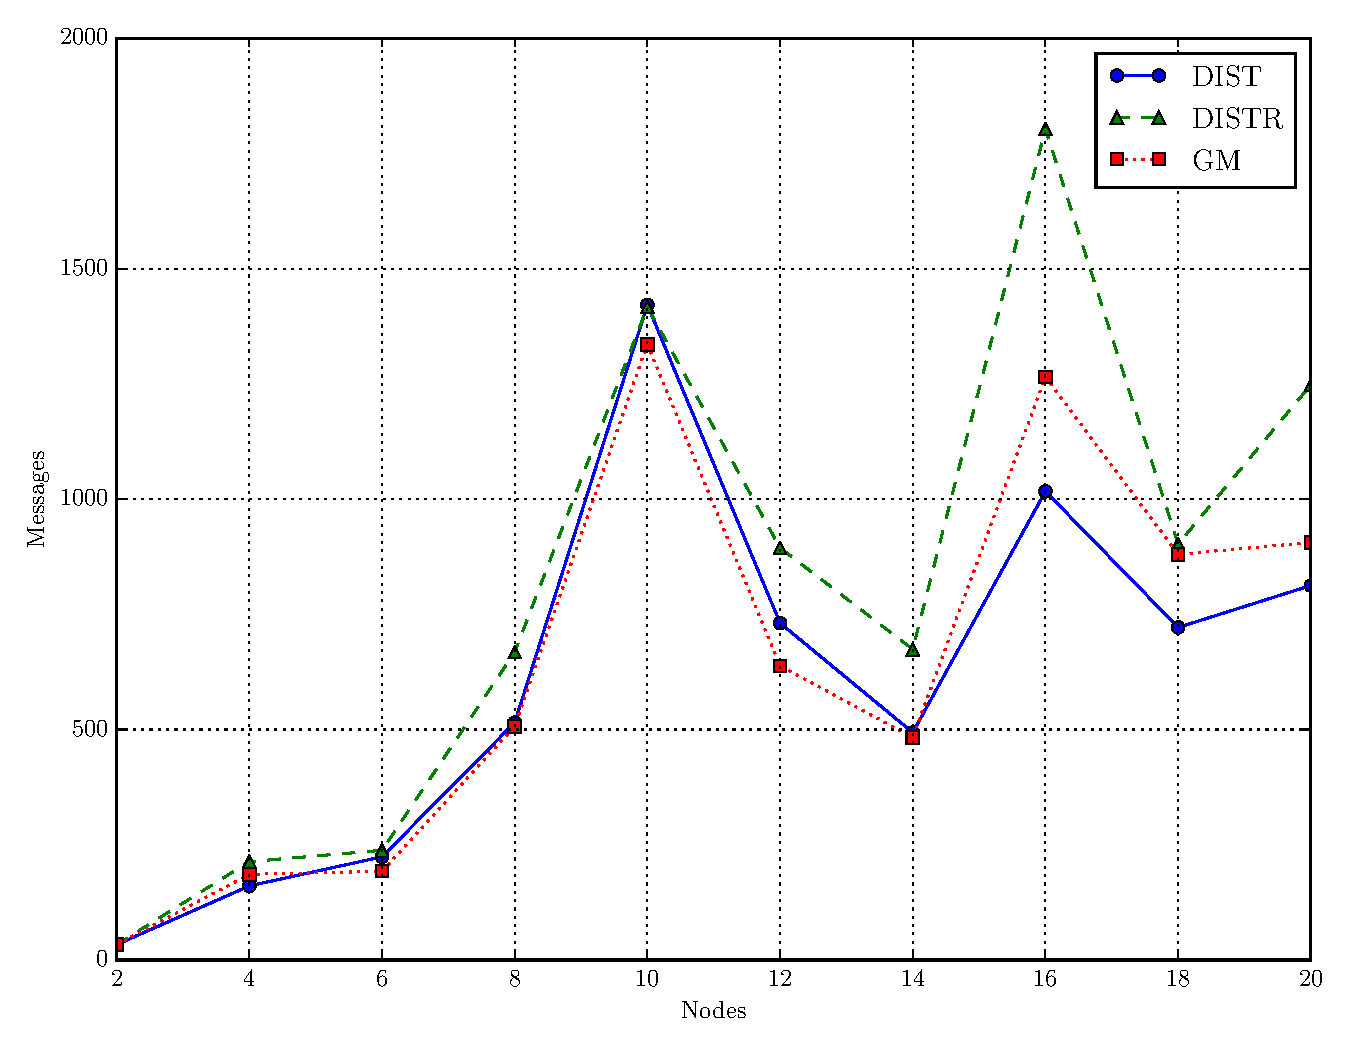
\includegraphics[scale=0.28, trim=4.5cm 0 0 0]{img/matching_msg_interweaving.pdf}
\caption{Local statistics streams of 8 nodes monitoring the variance of $NO_2$ air pollutant.} 
\end{subfigure}
\begin{subfigure}[t]{0.31\textwidth}
\centering
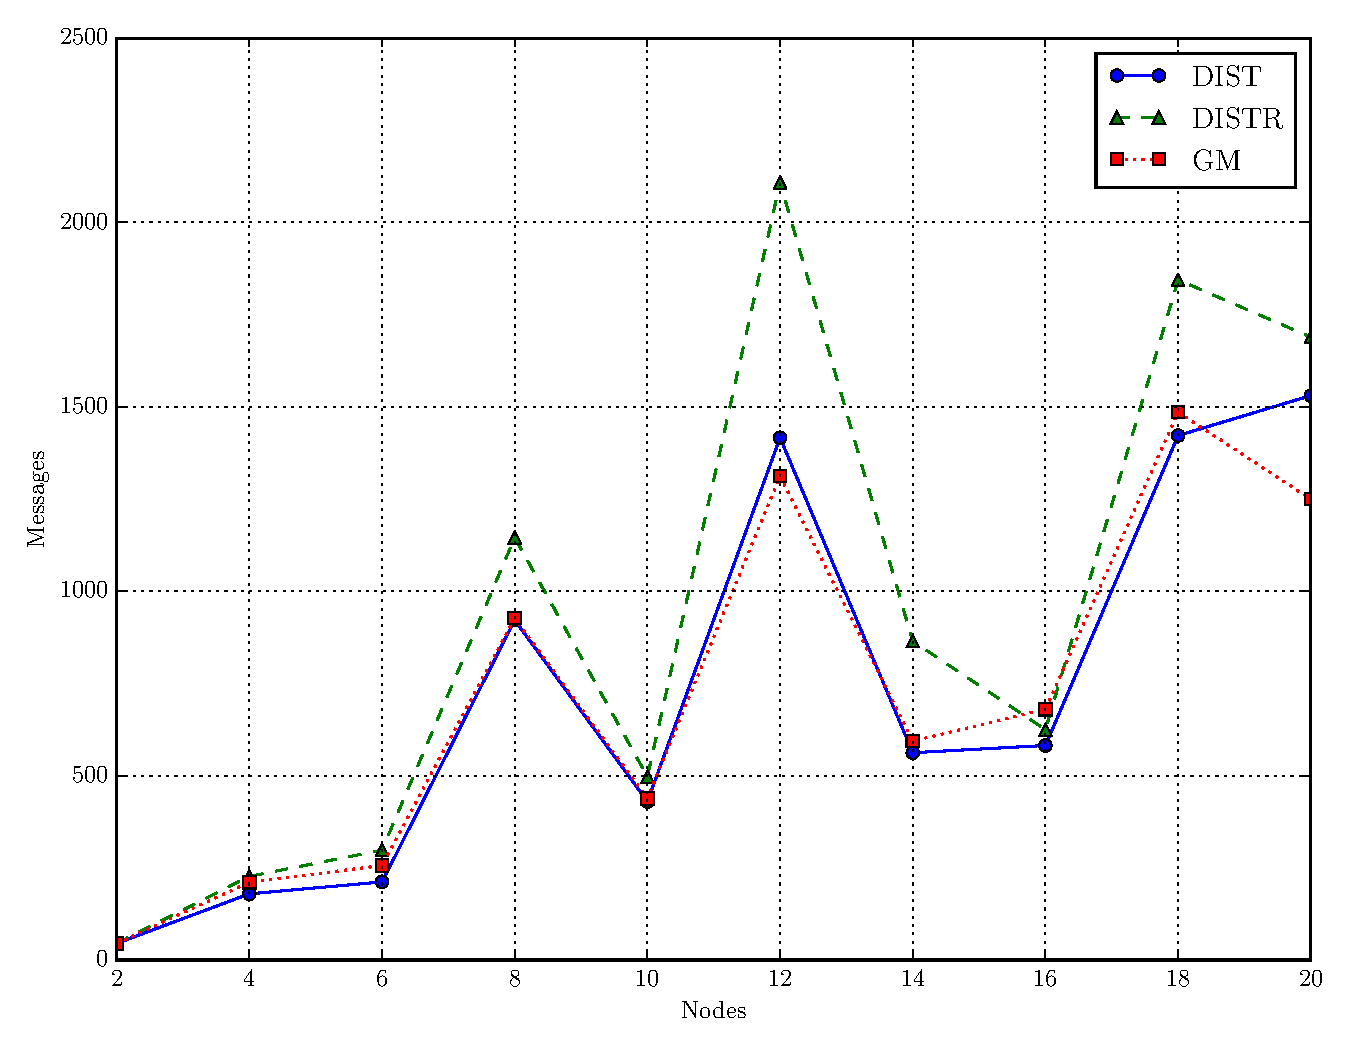
\includegraphics[scale=0.28]{img/matching_msg_noisyinterweaving.pdf}
\caption{Local statistics streams of 8 nodes monitoring the variance of $NO_2$ air pollutant.} 
\end{subfigure}
\vspace{0.5cm}
\caption{Streams of 8 nodes monitoring the variance of $NO_2$ air pollutant.}\label{fig:NO2_sq}
\end{figure*}
%%%%%%%%%%%%%%%%%%%%%%%%%%%%%%%%%%%%%%%%%%%%%%%%%%%%%%%%%%%%%%%%%%%%%%%%%%%%%%%%%%%%%%%%%%%



compare distance based node matching to distribution based node matching and the random selection algorithm with the classic balancing method

*images

\subsection{Balancing methods} \label{subsec:balComp}

compare classic balancing with heuristic balancing with random selection algorithm

*images

\subsection{Monitoring Synthetic Data} \label{subsec:mainComp}

compare classic random with heuristic distance based matching over a range of nodes, a range of window sizes and a range of orders for SG

*images

%TODO:actual data?
\subsection{Monitoring Air Quality Data} \label{subsec:actualComp}

compare classic random with heristic distance based matching for the actual data, over a range of nodes and sg parameters to check how it affects performance

actual data streams that have great variance and irregularities lead to poor proposed algorithm performance

*images
